\chapter{Diseño e implementación del sistema}
Este capítulo describe la arquitectura general del sistema y detalla cada uno de sus componentes, desde el montaje electrónico del CanSat hasta la visualización de los datos en tiempo real.

Se justifica la elección del hardware y software empleados, se explica el funcionamiento del código embebido, y se documenta la integración entre los distintos módulos del sistema: la Raspberry Pi, el backend en Spring Boot, la base de datos, el broker de eventos RabbitMQ y el frontend desarrollado en Flutter.

Finalmente, se presentan las pruebas realizadas para verificar el funcionamiento del sistema completo.


\section{Selección de componentes y tecnologías utilizadas}


Este apartado describe los principales elementos hardware y software empleados en el sistema.

La selección se ha basado en los requisitos técnicos del proyecto y en las conclusiones del análisis comparativo desarrollado en el capítulo anterior.

\begin{itemize}
    \item \textbf{Unidad de procesamiento:} se ha utilizado una~\cite{raspberrypi_zero2}.

    \begin{figure}[H]
        \centering
        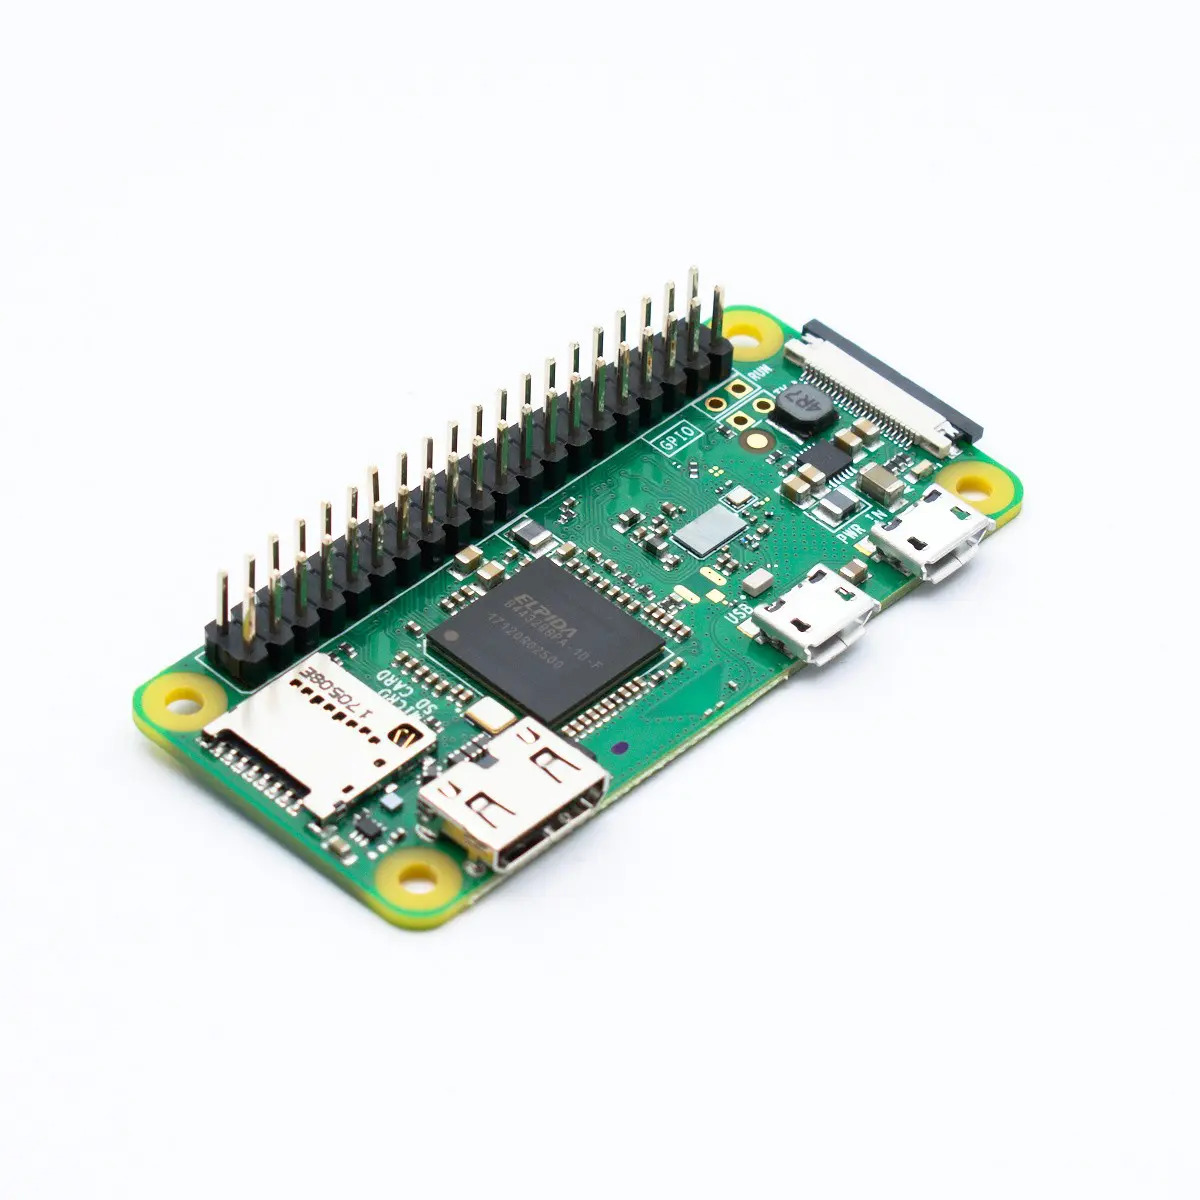
\includegraphics[width=0.2\textwidth]{Imagenes/Bitmap/ras2}
        \caption{Raspberry Pi Zero 2 W}
        \label{fig:ras2}
    \end{figure}

    Su capacidad para ejecutar Linux, capturar y codificar vídeo por hardware, y gestionar interfaces como I\textsuperscript{2}C, UART y CSI, la hacen adecuada para su integración directa en un CanSat sin necesidad de microcontroladores adicionales.
    \item \textbf{Sensor de presión barométrica:} el BMP388~\cite{adafruitBMP388} permite estimar la altitud mediante medición barométrica.
    Además de la presión atmosférica, proporciona la temperatura del entorno.
    Ofrece una precisión de ±8~Pa, bajo consumo y comunicación por I\textsuperscript{2}C.

    \begin{figure}[H]
        \centering
        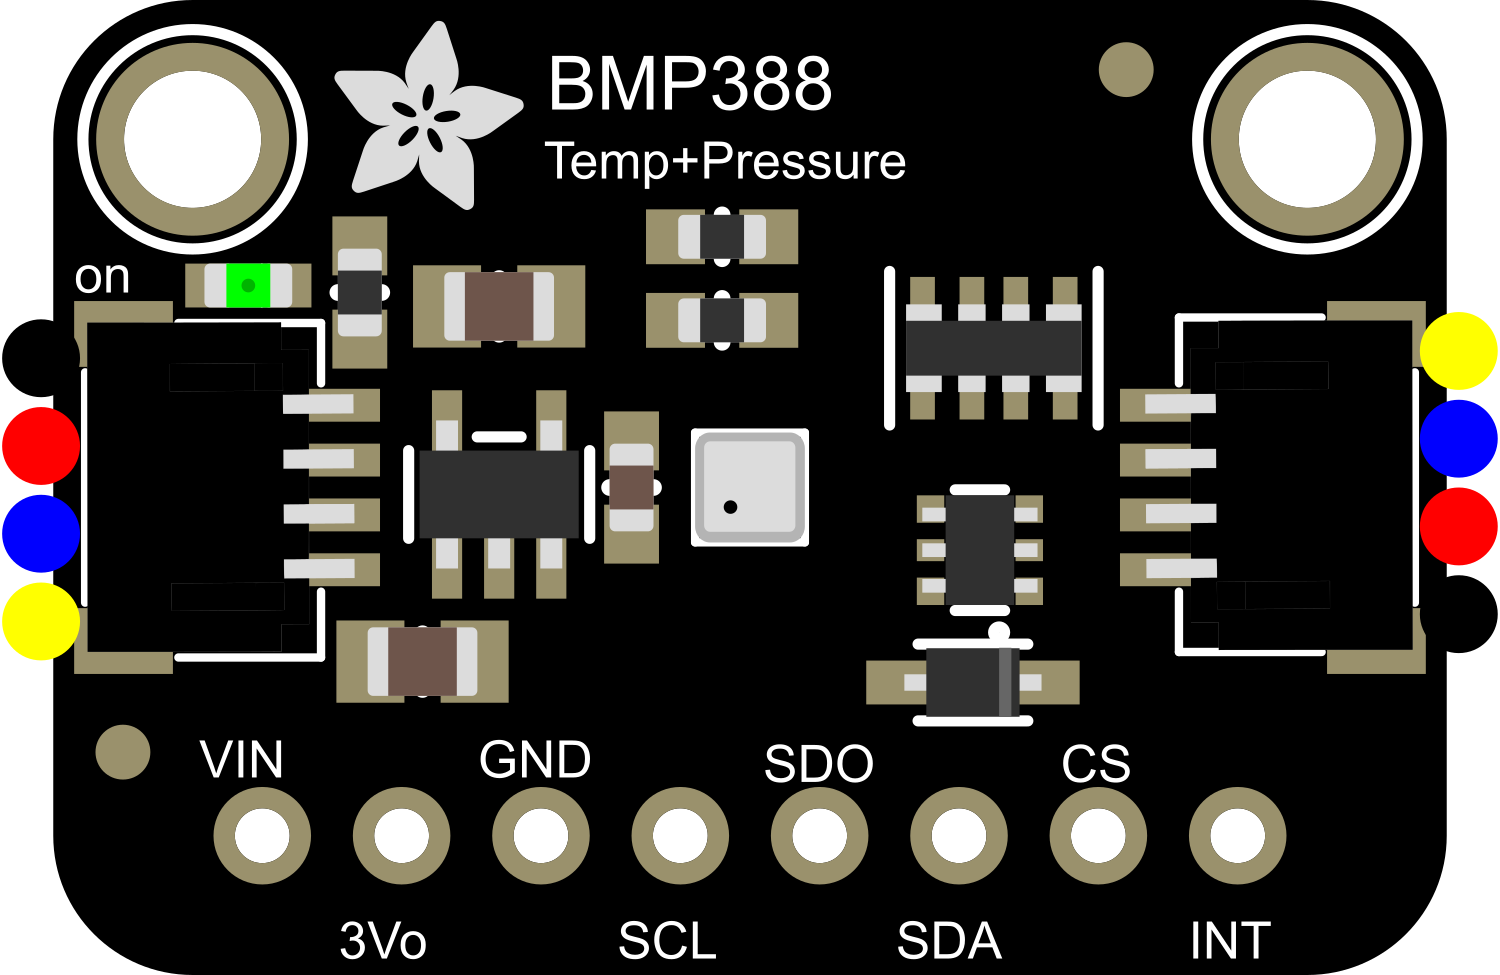
\includegraphics[width=0.4\textwidth]{Imagenes/Bitmap/bmp388}
        \caption{Sensor de presión barométrica bmp388}
        \label{fig:bmp388}
    \end{figure}

    \item \textbf{IMU:} Se ha empleado el BNO085~\cite{adafruitBNO085}, un sensor de 9 grados de libertad que combina acelerómetro, giroscopio y magnetómetro.
    Incorpora un procesador dedicado que realiza la fusión sensorial internamente y entrega directamente la orientación absoluta, lo que evita cálculos adicionales en la Raspberry Pi.

    \begin{figure}[H]
        \centering
        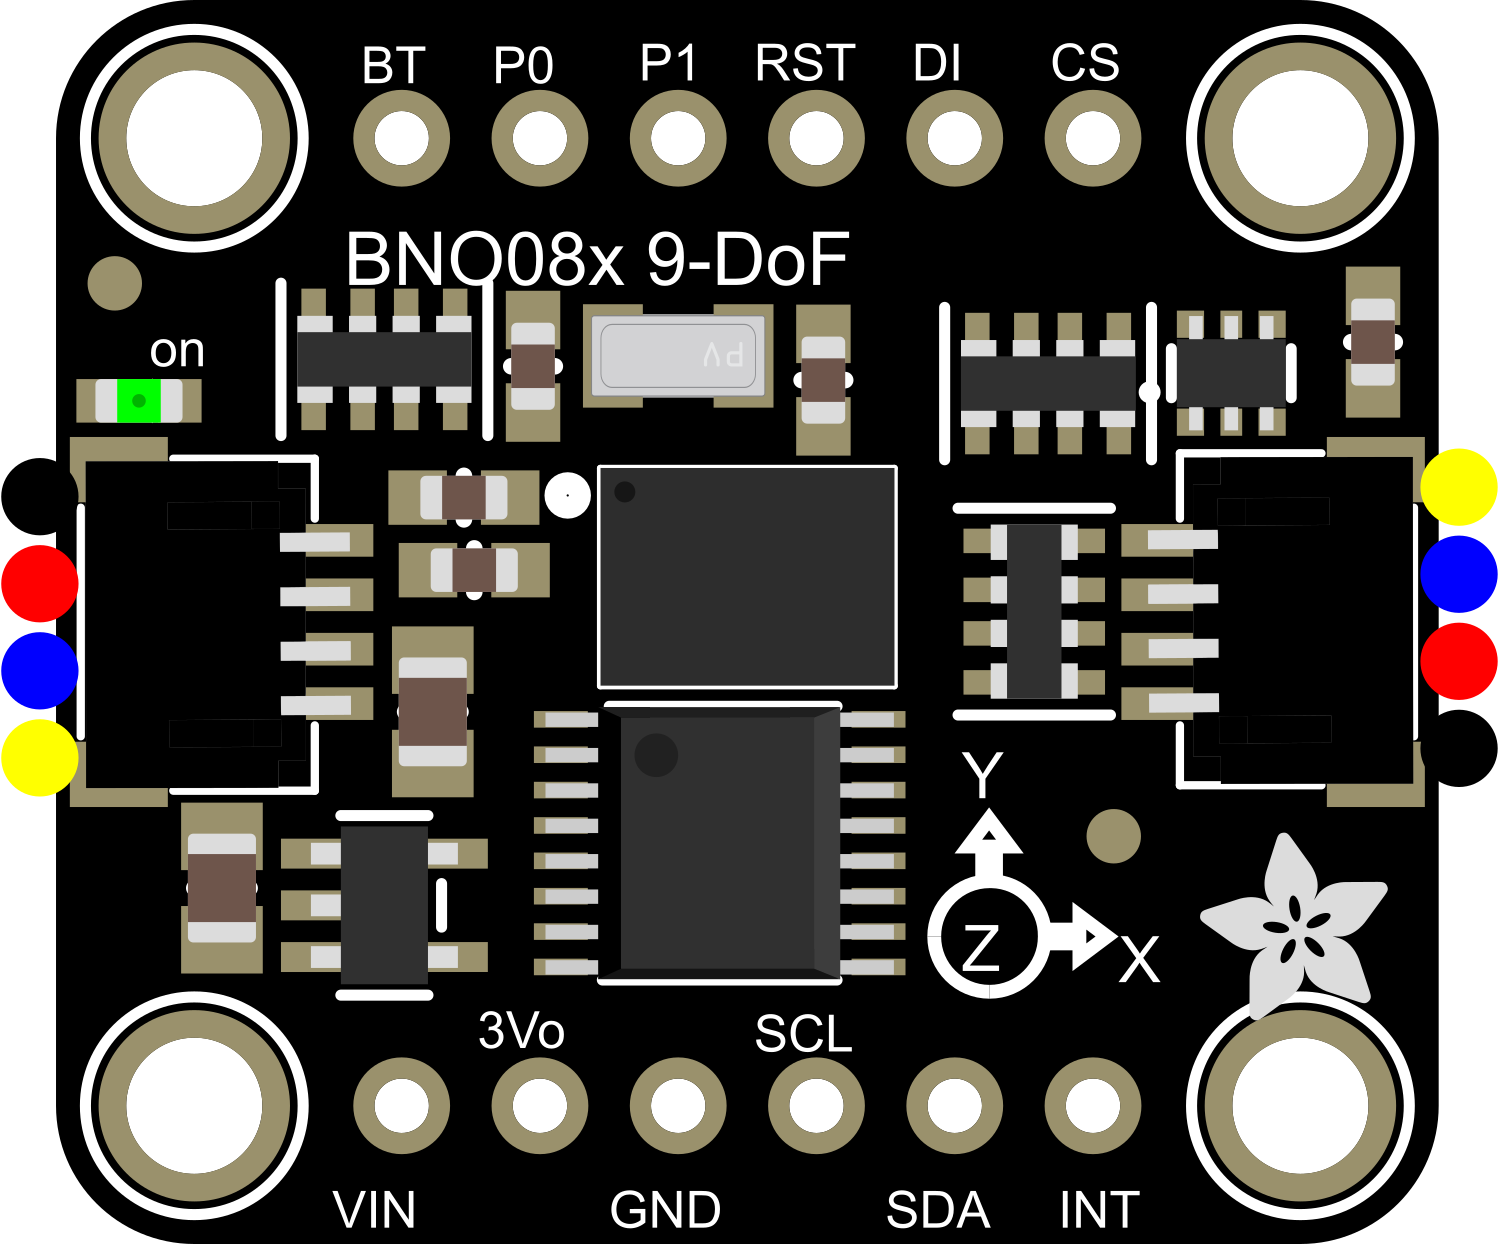
\includegraphics[width=0.4\textwidth]{Imagenes/Bitmap/bno085}
        \caption{IMU bno085}
        \label{fig:bno085}
    \end{figure}
    \item \textbf{GNSS:} se ha utilizado el módulo BN-880~\cite{bn880Module}, que integra un receptor GNSS con soporte para múltiples constelaciones (GPS, GLONASS, Galileo y BeiDou).
    Proporciona datos de posición, velocidad y altitud en tiempo real mediante interfaz UART. Incluye una antena activa integrada y una brújula electrónica.
    \begin{figure}[H]
        \centering
        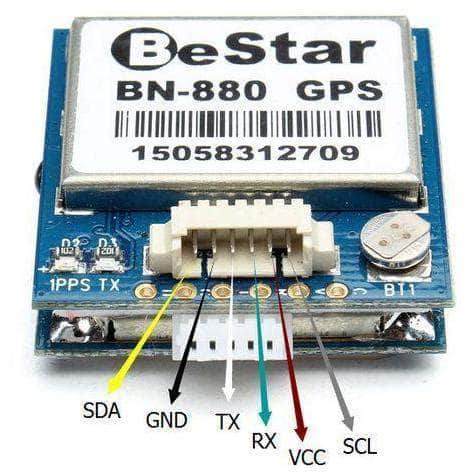
\includegraphics[width=0.4\textwidth]{Imagenes/Bitmap/bn-880}
        \caption{GPS bn-880}
        \label{fig:bn-880}
    \end{figure}
    \item \textbf{Cámara:} se utiliza el modelo oficial de la Raspberry Pi~\cite{raspiCamV2} con interfaz CSI. Permite la captura de vídeo codificado en H.264 mediante la GPU, sin comprometer el rendimiento del sistema.
    \begin{figure}[h]
        \centering
        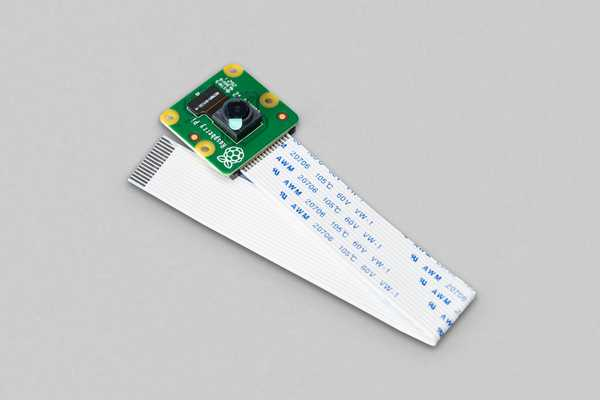
\includegraphics[width=0.4\textwidth]{Imagenes/Bitmap/rascamv2}
        \caption{Raspberry Pi Camera Module 2}
        \label{fig:rascamv2}
    \end{figure}
    \item \textbf{Transmisión de datos:} el sistema utiliza Wi-Fi si hay red disponible, en caso contrario el módulo LoRa E32-900T20D~\cite{ebyteE32}.
    Este módulo opera en 868~MHz y permite comunicación a larga distancia mediante UART.
    \begin{figure}[h]
        \centering
        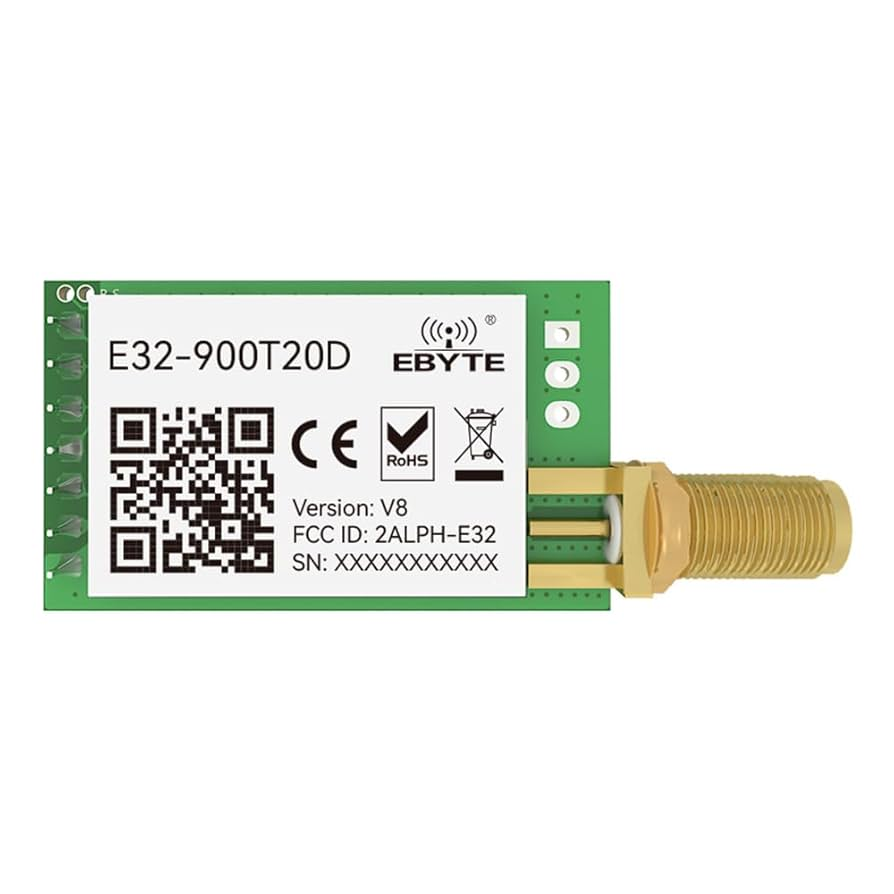
\includegraphics[width=0.4\textwidth]{Imagenes/Bitmap/lorae32}
        \caption{Módulo LoRa E32-900T20D}
        \label{fig:lorae32}
    \end{figure}

    \item \textbf{Antena LoRa:} se utiliza una antena externa de 868–915~MHz, con conector SMA macho, ganancia de 3~dBi e impedancia de 50~\(\Omega\).

    \begin{figure}[h]
        \centering
        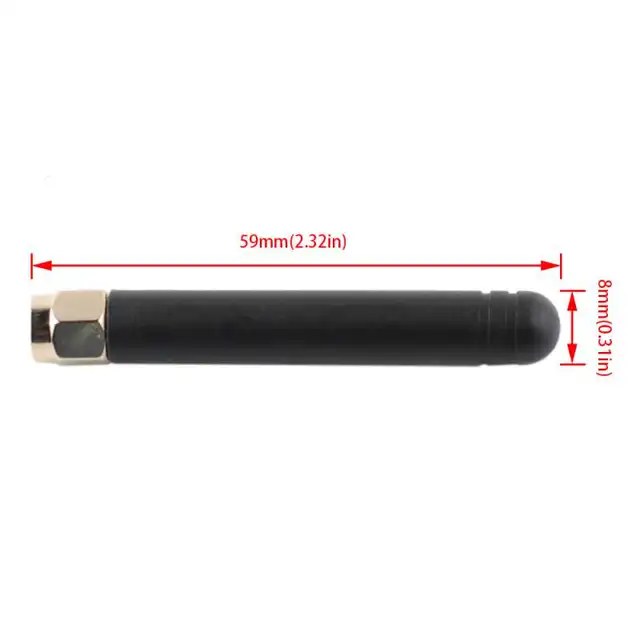
\includegraphics[width=0.4\textwidth]{Imagenes/Bitmap/antena_lora}
        \caption{Antena LoRa U.FL a SMA 868–915~MHz, 3~dBi}
        \label{fig:antena_lora}
    \end{figure}

    \item \textbf{Alimentación:} el sistema se alimenta mediante una batería recargable de ion de litio (Li-ion) tipo 18650 de 3{,}7~V conectada a un cargador MCP73871~\cite{mcp73871Datasheet}, que permite la recarga mediante panel solar y proporciona protección frente a sobrecarga, descarga profunda y cortocircuitos.

    Para obtener los 5~V requeridos por la Raspberry Pi, se emplea un convertidor elevador DC-DC ajustable (modelo VISSQH), que incrementa la tensión de entrada hasta una salida estabilizada.

    \begin{figure}[H]
        \centering
        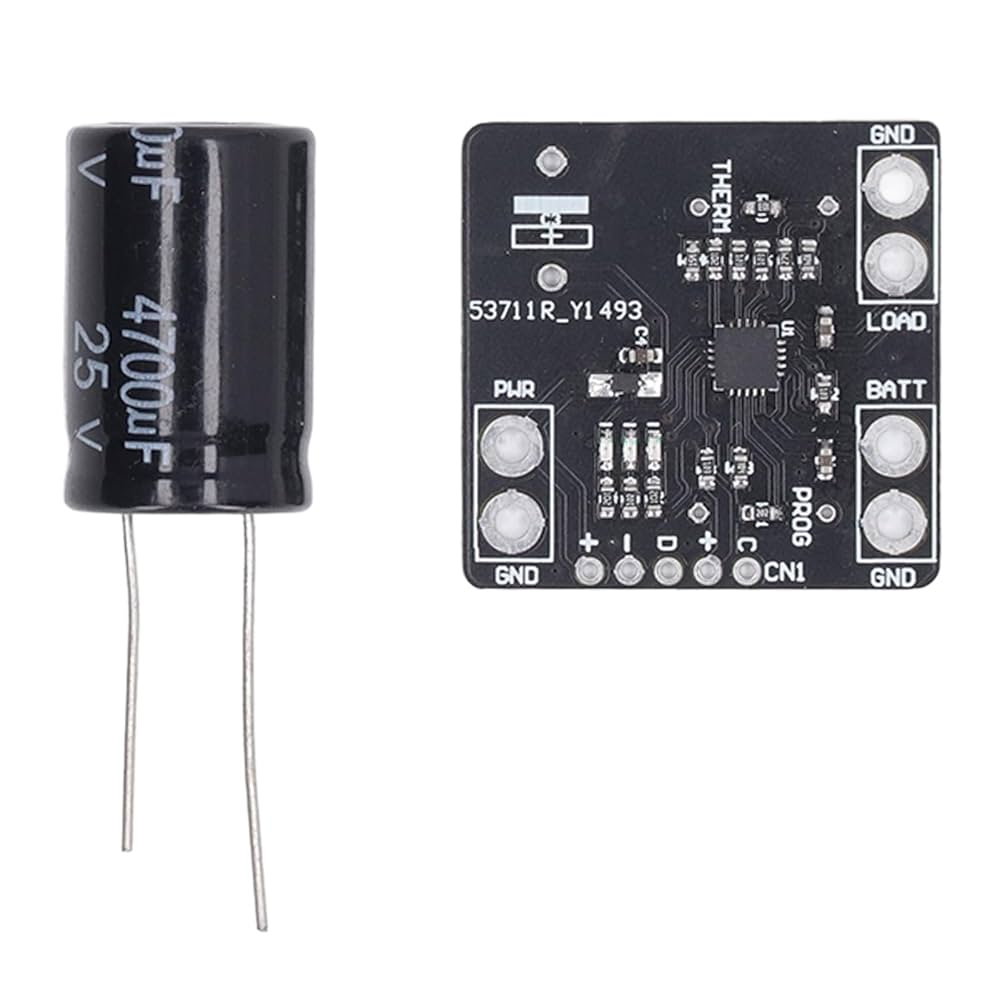
\includegraphics[width=0.4\textwidth]{Imagenes/Bitmap/mcp73871}
        \caption{Cargador MCP73871}
        \label{fig:mcp73871}
    \end{figure}
    \begin{figure}[H]
        \centering
        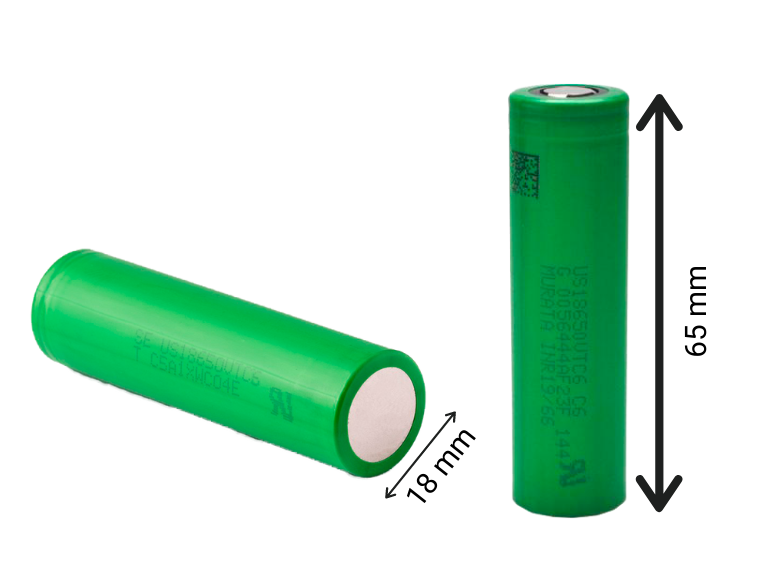
\includegraphics[width=0.4\textwidth]{Imagenes/Bitmap/18650}
        \caption{Batería 18650}
        \label{fig:18650}
    \end{figure}
    \item \textbf{Estación de tierra:} está formada por un receptor LoRa conectado mediante UART a una Raspberry Pi 4.

    Esta actúa como pasarela entre el CanSat y el sistema de mensajería RabbitMQ, reenviando los datos recibidos a través de LoRa.

    \item \textbf{Software embebido:} tanto la Raspberry Pi usada en el CanSat como la de la estación de tierra ejecutan scripts desarrollados en Python.

    \item \textbf{Software del sistema:} el backend está desarrollado en Java utilizando el framework Spring Boot, que facilita la construcción de servicios web REST y la integración con sistemas de mensajería.

    Para el intercambio de mensajes se emplea RabbitMQ, un sistema de colas que implementa el protocolo AMQP.

    La persistencia de datos se gestiona con PostgreSQL, un sistema de gestión de bases de datos relacional.

    La interfaz de usuario está implementada en Flutter, un framework multiplataforma desarrollado en Dart, y establece la comunicación en tiempo real mediante WebSocket utilizando el protocolo STOMP.
\end{itemize}


\section{Arquitectura general del sistema}
La arquitectura del sistema se organiza en tres bloques principales: el CanSat, la estación de tierra y la infraestructura de backend y visualización web.

Esta arquitectura sigue un enfoque orientado a eventos, en el que los datos generados por el CanSat son publicados y transmitidos hacia los consumidores mediante mecanismos de mensajería asincrónica.

Los tres componentes principales son:

\begin{itemize}
    \item \textbf{CanSat: }integra sensores, módulo GNSS, cámara y comunicaciones.

    Una Raspberry Pi Zero 2 W adquiere y empaqueta los datos de telemetría para su envío.
    Cuando hay red Wi‑Fi disponible, los eventos se publican directamente en un broker RabbitMQ. En caso contrario, los datos se transmiten mediante LoRa a la estación de tierra.

    Todos los datos de telemetría adquiridos por los sensores se guardan de manera local en formato JSON.
    En cuanto a la retransmisión de vídeo en tiempo real, solo se realiza cuando está conectado a una red Wi-Fi, en caso contrario, el vídeo se guarda en la memoria de la Raspberry Pi.

    \item \textbf{Estación de tierra: }compuesta por una Raspberry Pi 4 conectada al receptor LoRa mediante UART.

    Ejecuta un script en Python que interpreta los paquetes recibidos y los reenvía al broker RabbitMQ a través de la red.

    Esta estación actúa como pasarela cuando no hay conectividad directa entre el CanSat y la infraestructura de backend en los casos en los que no existe conexión directa mediante red.

    \item \textbf{Infraestructura de visualización: } esta infraestructura está formada por varios componentes:
    \begin{itemize}
        \item \textbf{RabbitMQ: } recibe los eventos de telemetría desde la estación de tierra o directamente desde el CanSat y los transmite al backend.
        \item \textbf{Backend: } se encarga de consumir los eventos con los datos de telemetría que llegan desde RabbitMQ,
        guardarlos en la base de datos para su posterior descarga, y emitir los eventos hasta el frontend utilizando websockets.
        \item \textbf{Base de datos: } se trata de una base de datos relacional PostgreSQL, en ella se guardan todos los eventos de telemetría asociados a su fecha de recepción.
        \item \textbf{Frontend: } es una aplicación web desarrollada en Flutter, cuenta con distintos tipos de gráficas para visualizar los datos del CanSat en tiempo real a través de WebSockets.
        \item \textbf{Servidor de vídeo en tiempo real:} recibe el flujo de vídeo codificado desde el CanSat mediante el protocolo RTMP y lo adapta para su reproducción en navegadores web.
        La transmisión solo se realiza cuando hay conectividad Wi‑Fi disponible.
    \end{itemize}
    Para mejorar la portabilidad y facilitar el despliegue de la infraestructura en distintos entornos, todos los servicios del backend, la base de datos, el broker de mensajería y el servidor de vídeo se han contenerizado utilizando Docker.
\end{itemize}
\begin{figure}[H]
    \centering
    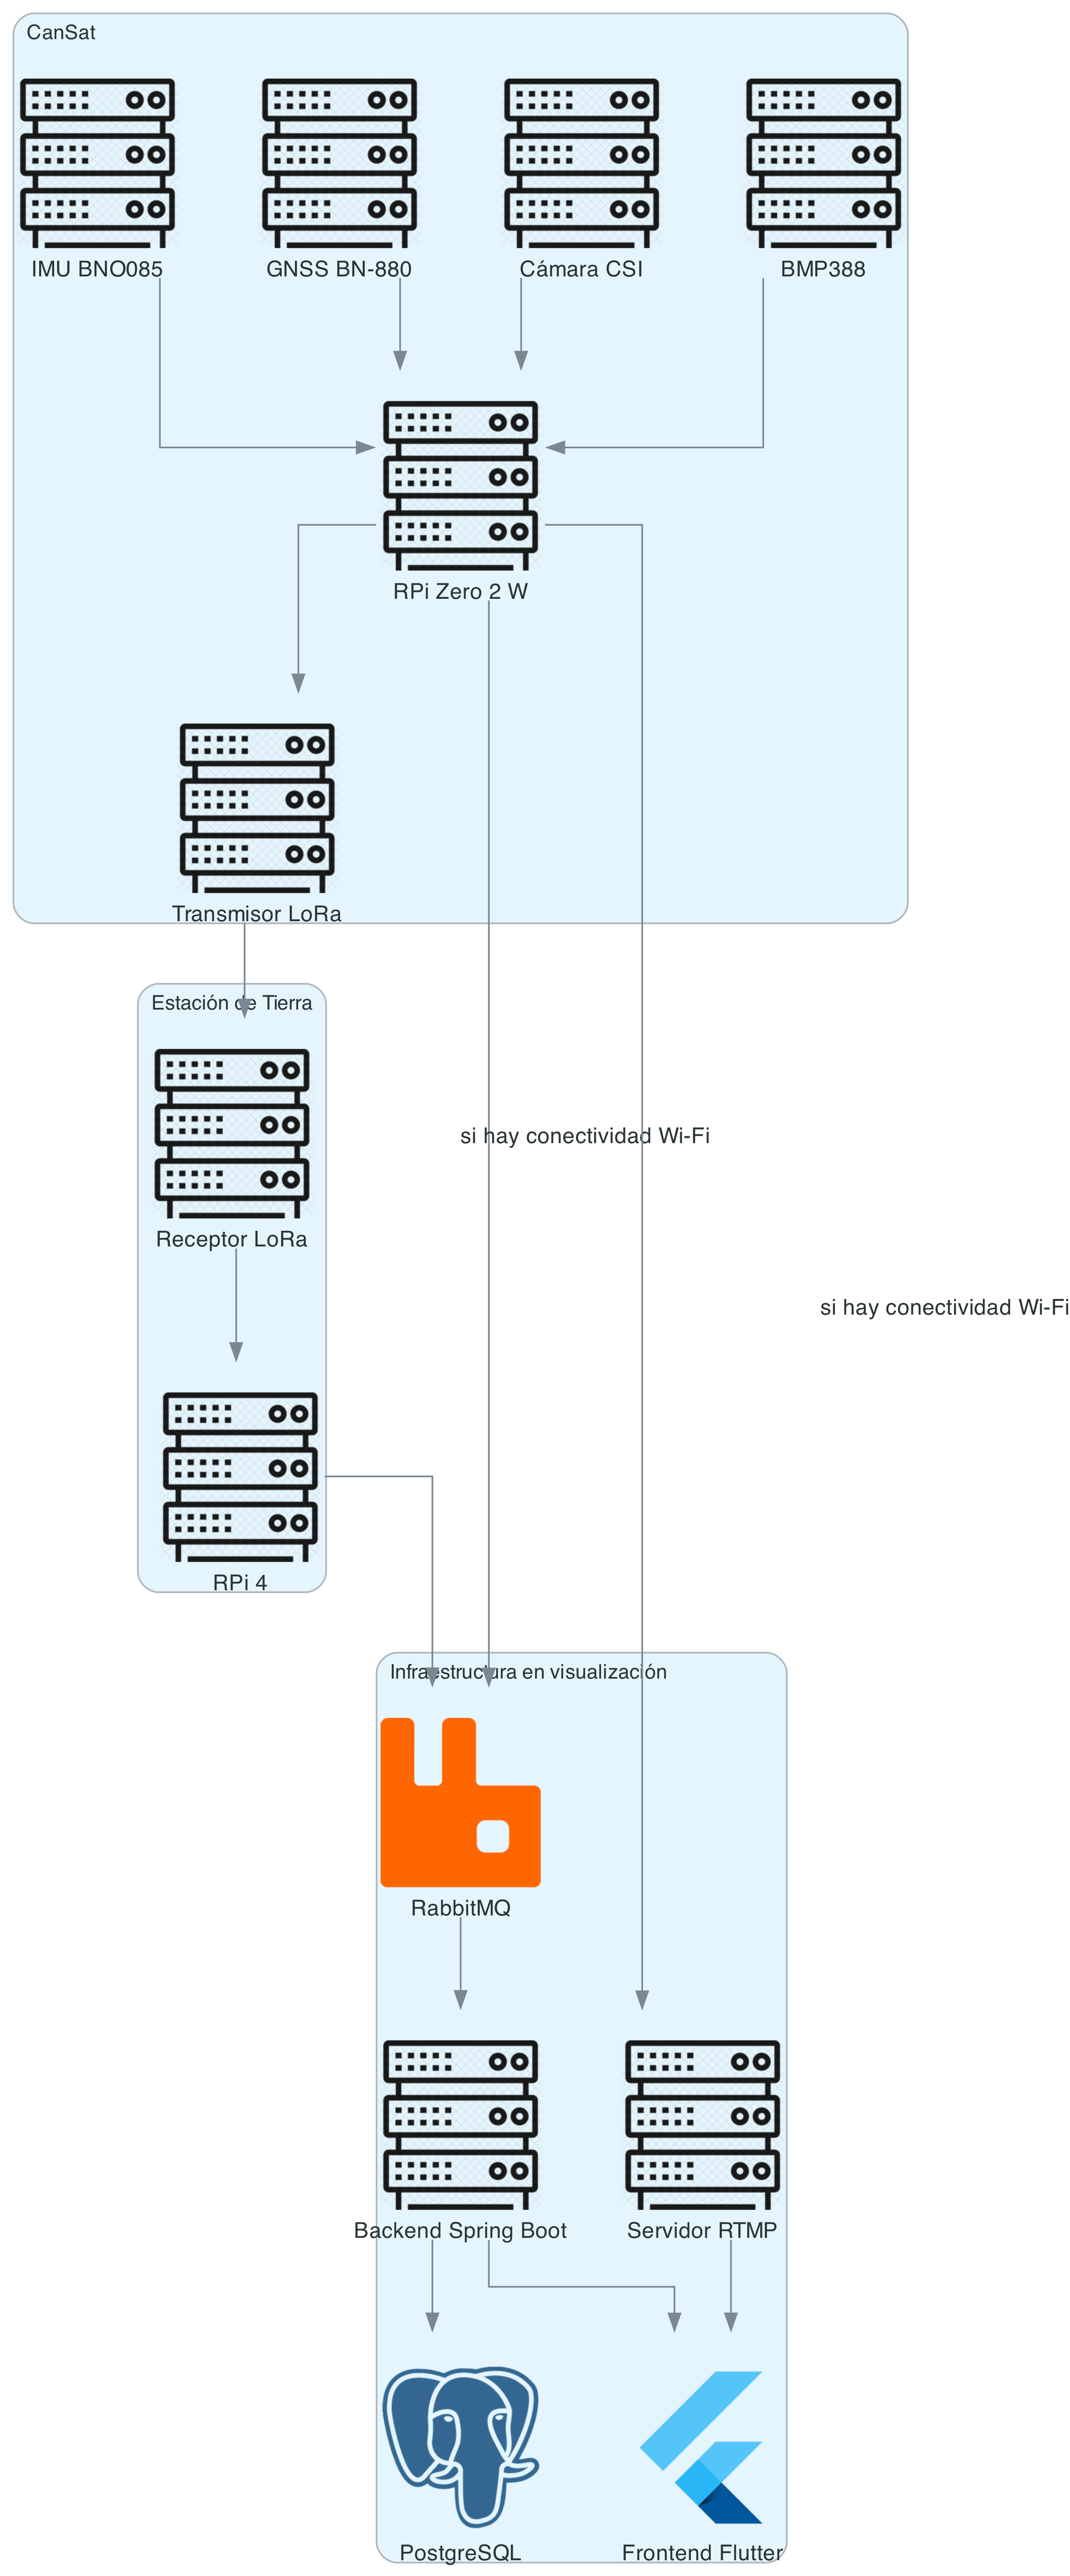
\includegraphics[width=0.51\textwidth]{Imagenes/Bitmap/cansat_architecture}
    \caption{Arquitectura general del sistema}
    \label{fig:cansat_architecture}
\end{figure}


\section{Montaje electrónico del CanSat}
El montaje electrónico se realizó inicialmente sobre una protoboard, con el objetivo de validar las conexiones y el funcionamiento de los distintos módulos durante la fase de desarrollo.

Cada componente fue integrado mediante cableado directo a la Raspberry Pi Zero 2 W, usando las interfaces específicas de cada uno (UART, I\textsuperscript{2}C).

A continuación, se describen las conexiones realizadas entre los distintos periféricos y la Raspberry Pi, incluyendo los pines utilizados y las interfaces empleadas.

\begin{itemize}
    \item \textbf{Sensor de presión BMP388:} utiliza la interfaz I\textsuperscript{2}C.
    \begin{itemize}
        \item SDA: GPIO~2 (pin físico~3)
        \item SCL: GPIO~3 (pin físico~5)
        \item Alimentación: 5~V (pin físico~2)
        \item GND: pin físico~6
    \end{itemize}

    \item \textbf{IMU BNO085:} también conectada por I\textsuperscript{2}C en el mismo bus que el BMP388.
    \begin{itemize}
        \item SDA: GPIO~2 (pin físico~3)
        \item SCL: GPIO~3 (pin físico~5)
        \item Alimentación: 5~V (pin físico~2)
        \item GND: pin físico~6
    \end{itemize}

    \item \textbf{Módulo LoRa E32-900T20D:} comunica por UART.
    \begin{itemize}
        \item TX del módulo → RX de la Pi: GPIO~15 (pin físico~10)
        \item RX del módulo ← TX de la Pi: GPIO~14 (pin físico~8)
        \item Alimentación: 5~V (pin físico~2)
        \item GND: pin físico~6
        \item Pines M0 y M1: conectados respectivamente a los GPIO~23 (pin físico~16) y GPIO~24 (pin físico~18) de la Raspberry Pi, lo que permite gestionar el modo de operación del módulo desde software.
        \item Conexión de antena: la antena externa se conecta al conector SMA hembra del módulo LoRa, permitiendo la comunicación en la banda de 868–915~MHz.
    \end{itemize}
    \begin{figure}[H]
        \centering
        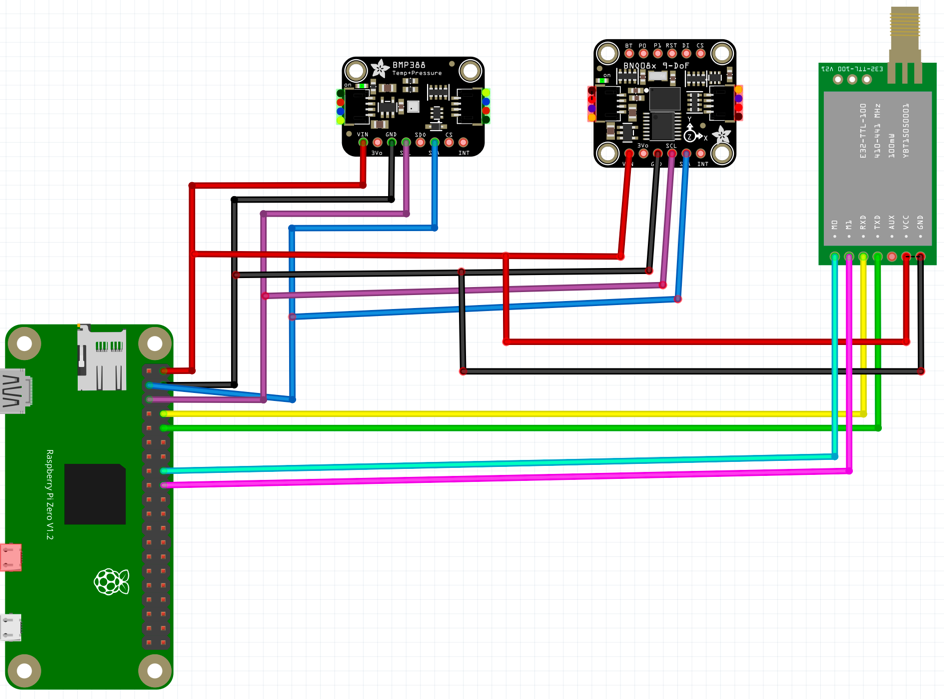
\includegraphics[width=0.7\textwidth]{Imagenes/Bitmap/conexion_sensores}
        \caption{Diagrama de conexión de los sensores y módulo LoRa}
        \label{fig:conexion_sensores}
    \end{figure}
    \item \textbf{GNSS BN-880:} comunica por UART. Dado que la Raspberry Pi Zero 2~W solo dispone de un puerto UART hardware accesible por GPIO (usado en este caso por el módulo LoRa),
    se ha optado por conectar el BN-880 a través de un adaptador USB a UART.

    El módulo utilizado es un conversor basado en el chip CP2102, que se conecta al puerto micro-USB de la Raspberry Pi y proporciona una interfaz UART adicional accesible desde el sistema operativo como un puerto /dev/ttyUSB0.

    Dado el espacio reducido disponible, se ha modificado el adaptador CP2102 retirando el conector USB macho original y sustituyéndolo por un conector micro-USB macho, soldado directamente a la placa.
    Esto permite conectarlo al puerto micro-USB de datos de la Raspberry Pi de forma más compacta, sin necesidad de adaptadores adicionales.

    \begin{itemize}
        \item TX del GNSS → RX del adaptador
        \item RX del GNSS ← TX del adaptador
        \item Alimentación: 5~V conectado al pin VCC del adaptador
        \item GND: pin físico~14 conectado al GND del adaptador
        \item Conexión de datos: vía micro-USB del adaptador al puerto USB de la Raspberry Pi
    \end{itemize}
    \begin{figure}[H]
        \centering
        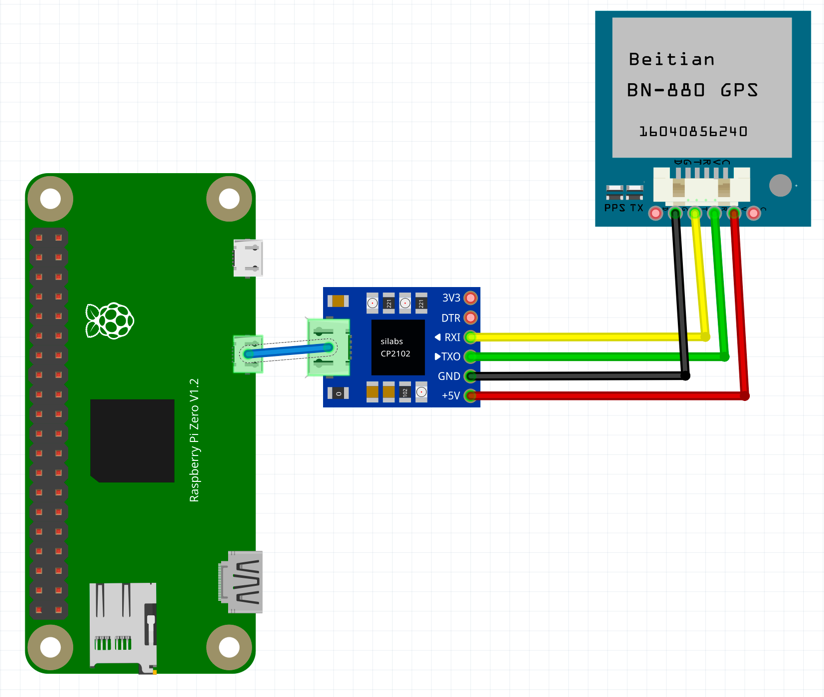
\includegraphics[width=0.7\textwidth]{Imagenes/Bitmap/conexion_gps}
        \caption{Diagrama de conexión del módulo GNSS BN-880 mediante el adaptador CP2102 }
        \label{fig:conexion_gps}
    \end{figure}
    \item \textbf{Cargador MCP73871:} es el encargado de gestionar la alimentación del sistema y la recarga de la batería.

    Este módulo permite cargar una batería de ion de litio y, simultáneamente, alimentar el sistema, conmutando automáticamente entre la entrada de alimentación externa y la batería según su disponibilidad.


    \begin{itemize}
        \item \textbf{Entrada de carga:} al conector USB-C hembra del módulo se conecta una entrada de alimentación externa.

        En este caso, se utilizan tres paneles solares de 2~V conectados en serie, cuyo cableado termina en un conector USB-C macho compatible con la entrada del cargador.

        \item \textbf{Conexión de la batería:} una batería de ion de litio de 3{,}7~V (tipo 18650) se conecta directamente a los terminales BAT+ y BAT- del módulo.

        Esta conexión permite tanto la carga de la batería como el suministro de energía al sistema cuando no hay entrada externa disponible.

        \item \textbf{Salida VBUS:} el terminal VBUS proporciona la tensión de salida activa en cada momento (procedente de la entrada USB-C o de la batería).

        Esta salida no está regulada y puede variar entre 3{,}7~V y 5{,}5~V, por lo que se conecta a un convertidor elevador (boost converter) que estabiliza la tensión a 5~V.

        La salida del boost se conecta al pin físico~2 (5~V) de la Raspberry Pi, y su masa al pin físico~39 (GND), proporcionando alimentación estable a todo el sistema.
    \end{itemize}
    \begin{figure}[H]
        \centering
        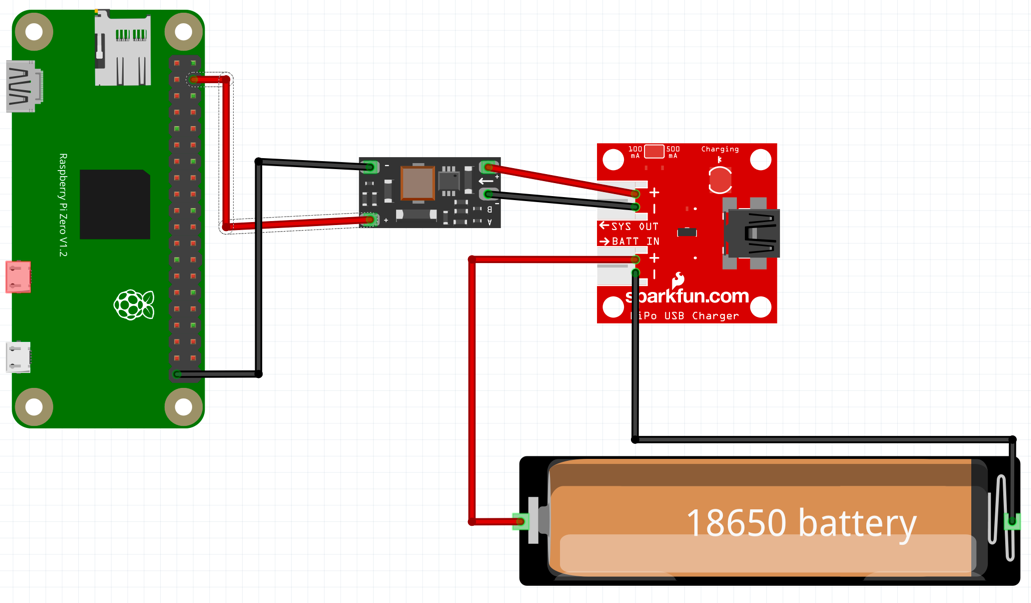
\includegraphics[width=0.7\textwidth]{Imagenes/Bitmap/conexion_cargador}
        \caption{Diagrama de conexión del cargador MCP73871 y booster}
        \label{fig:conexion_cargador}
    \end{figure}
    \item \textbf{Cámara CSI:} conectada directamente al puerto CSI (Camera Serial Interface) de la Raspberry Pi Zero 2 W mediante un cable plano.

    El puerto CSI es una interfaz específica para cámaras que permite transmitir vídeo sin utilizar pines GPIO.
    Además, proporciona tanto la alimentación como la señal de datos a través del propio conector.
\end{itemize}

\begin{table}[H]
    \centering
    \begin{tabular}{|l|l|l|l|}
        \hline
        \textbf{Módulo}     & \textbf{Función}     & \textbf{GPIO} & \textbf{Pin físico} \\ \hline
        BMP388              & SDA                  & GPIO 2        & 3                   \\ \cline{2-4}
        & SCL                  & GPIO 3        & 5                   \\ \cline{2-4}
        & VCC                  & -             & 1 (3.3 V)           \\ \cline{2-4}
        & GND                  & -             & 6                   \\ \hline
        BNO085              & SDA                  & GPIO 2        & 3                   \\ \cline{2-4}
        & SCL                  & GPIO 3        & 5                   \\ \cline{2-4}
        & VCC                  & -             & 1 (3.3 V)           \\ \cline{2-4}
        & GND                  & -             & 6                   \\ \hline
        LoRa E32-900T20D    & TX                   & GPIO 15       & 10                  \\ \cline{2-4}
        & RX                   & GPIO 14       & 8                   \\ \cline{2-4}
        & M0                   & GPIO 23       & 16                  \\ \cline{2-4}
        & M1                   & GPIO 24       & 18                  \\ \cline{2-4}
        & VCC                  & -             & 1 (5 V)             \\ \cline{2-4}
        & GND                  & -             & 6                   \\ \hline
        GNSS BN-880         & TX → RX del CP2102   & -             & -                   \\ \cline{2-4}
        & RX ← TX del CP2102   & -             & -                   \\ \cline{2-4}
        & VCC → VCC del CP2102 & -             & -                   \\ \cline{2-4}
        & GND → GND del CP2102 & -             & -                   \\ \hline
        Adaptador CP2102    & UART USB             & -             & Puerto USB (micro)  \\ \hline
        MCP73871 (cargador) & Entrada (USB-C)      & -             & -                   \\ \cline{2-4}
        & Salida a booster     & -             & -                   \\ \cline{2-4}
        & Boost out → Pi       & -             & 2 (5 V), 39 (GND)   \\ \hline
        Cámara CSI          & Datos + alimentación & -             & CSI                 \\ \hline
    \end{tabular}
    \caption{Resumen de conexiones de los periféricos a la Raspberry Pi Zero 2 W}
    \label{tab:resumen_conexiones}
\end{table}



A continuación se describe también el montaje de la estación de tierra, formada por un módulo LoRa conectado a una Raspberry Pi 4 a través de la interfaz UART:

\begin{itemize}
    \item TX del módulo → RX de la Pi: GPIO~15 (pin físico~10)
    \item RX del módulo ← TX de la Pi: GPIO~14 (pin físico~8)
    \item Pines M0 y M1: conectados respectivamente a los GPIO~23 (pin físico~16) y GPIO~24 (pin físico~18) de la Raspberry Pi, lo que permite gestionar el modo de operación del módulo desde software.
    \item Alimentación: 5~V (pin físico~2)
    \item GND: pin físico~6
    \item Conexión de antena: la antena externa se conecta al conector SMA hembra del módulo LoRa, permitiendo la comunicación en la banda de 868–915~MHz.

\end{itemize}

\begin{figure}[H]
    \centering
    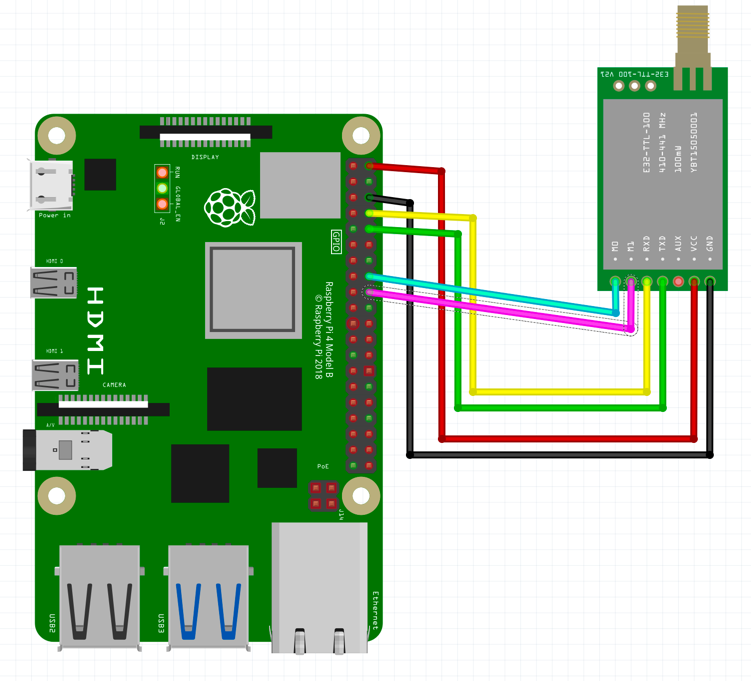
\includegraphics[width=0.7\textwidth]{Imagenes/Bitmap/conexion_ground}
    \caption{Diagrama de conexión de la estación de tierra con Raspberry Pi 4 y módulo LoRa}
    \label{fig:conexion_ground}
\end{figure}

\begin{table}[H]
    \centering
    \renewcommand{\arraystretch}{1.2}
    \begin{tabular}{|l|l|l|l|}
        \hline
        \textbf{Elemento} & \textbf{Función} & \textbf{GPIO} & \textbf{Pin físico} \\ \hline
        LoRa E32-900T20D  & TX → RX de la Pi & GPIO 15       & 10                  \\ \cline{2-4}
        & RX ← TX de la Pi & GPIO 14       & 8                   \\ \cline{2-4}
        & M0               & GPIO 23       & 16                  \\ \cline{2-4}
        & M1               & GPIO 24       & 18                  \\ \cline{2-4}
        & VCC              & --            & 2 (5 V)             \\ \cline{2-4}
        & GND              & --            & 6                   \\ \hline
    \end{tabular}
    \caption{Conexiones del módulo LoRa a la Raspberry Pi 4 en la estación de tierra}
    \label{tab:conexiones_ground_pi4}
\end{table}


Tras verificar el correcto funcionamiento de todas las conexiones en la protoboard, se procedió a su traslado a una placa PCB,
diseñada específicamente teniendo en cuenta las dimensiones y restricciones del CanSat.

\begin{figure}[H]
    \centering
    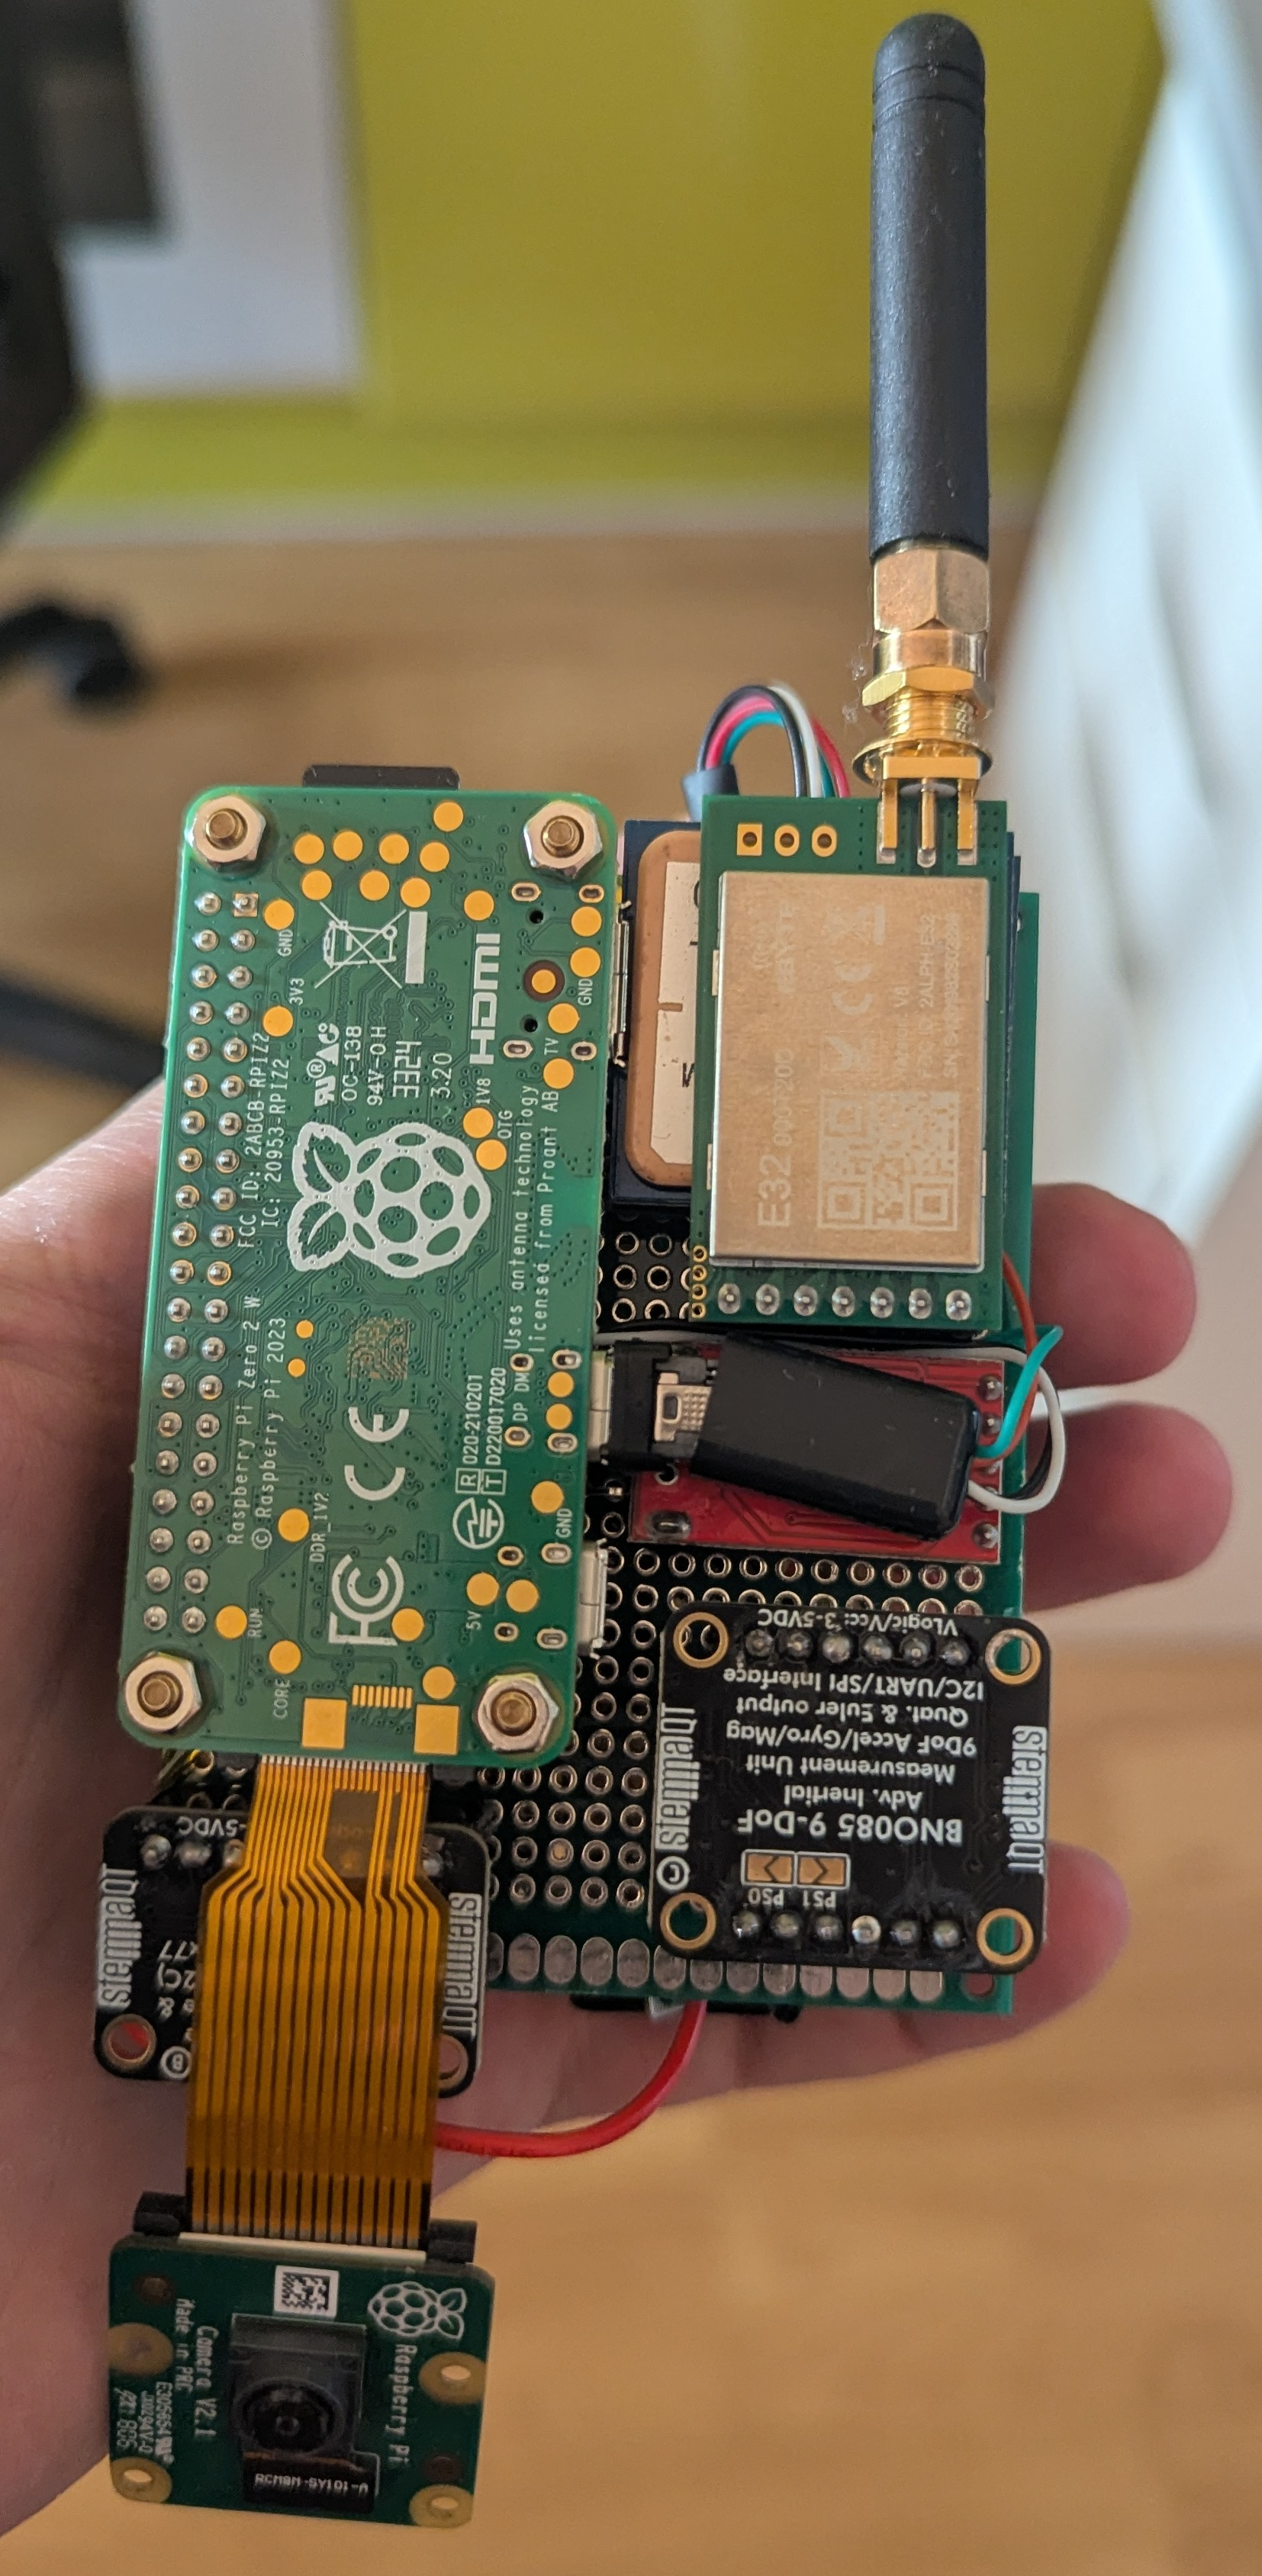
\includegraphics[width=0.3\textwidth]{Imagenes/Bitmap/pcb_montaje_frontal}
    \caption{Montaje final del sistema en la PCB (vista frontal)}
    \label{fig:pcb_montaje_frontal}
\end{figure}

\begin{figure}[H]
    \centering
    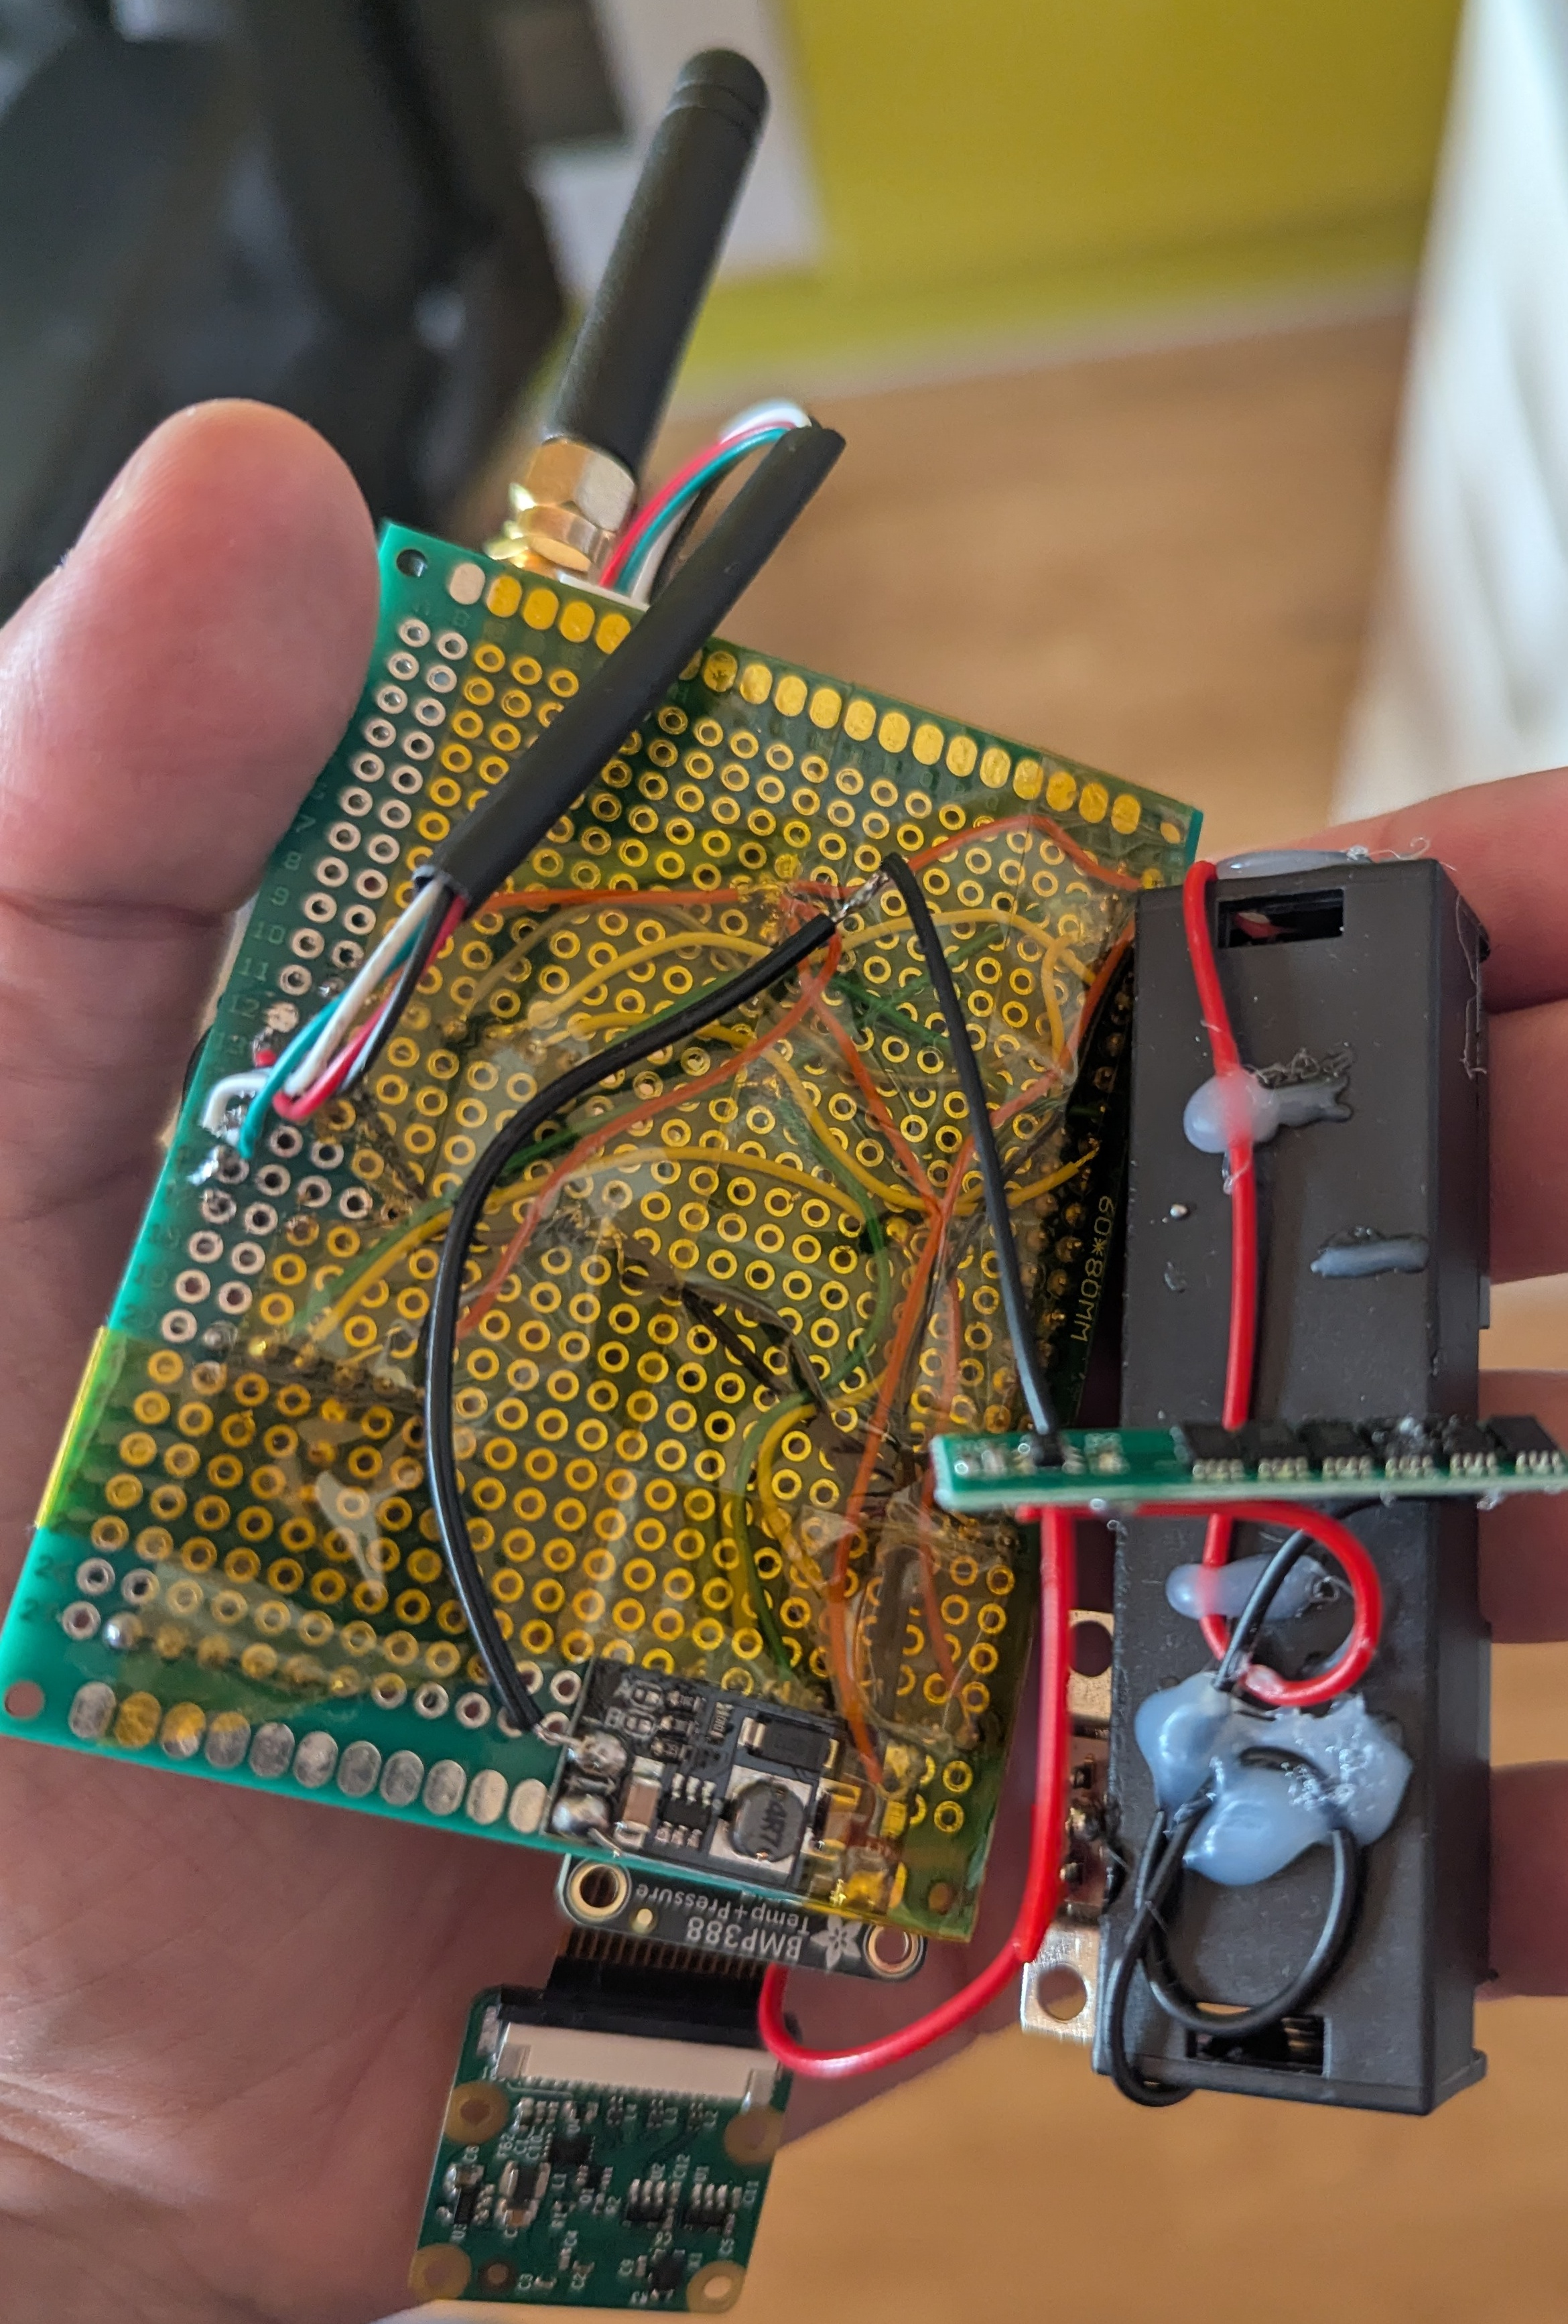
\includegraphics[width=0.5\textwidth]{Imagenes/Bitmap/pcb_montaje_trasero}
    \caption{Montaje final del sistema en la PCB (vista superior)}
    \label{fig:montaje_trasero}
\end{figure}


\section{Código embebido en la Raspberry Pi}

El código embebido desarrollado para la Raspberry Pi Zero 2~W está implementado en Python y se encarga de gestionar de forma concurrente la captura de vídeo, la adquisición de datos de sensores, el envío de eventos de telemetría por LoRa, y la publicación online a través de RabbitMQ.

El flujo de inicialización del sistema embebido sigue los siguientes pasos:

\begin{itemize}
    \item Esperar una conexión a internet durante 30 segundos para saber si debe enviar los datos mediante LoRa o publicarlos directamente en la cola de RabbitMQ.
    \item Crear una carpeta local donde se almacenarán los datos y vídeos generados, con nombre basado en la fecha y hora de arranque.
    \item Iniciar los módulos de captura de vídeo y envío de telemetría en hilos independientes.
\end{itemize}

\subsection{Captura de vídeo en tiempo real}

La clase \texttt{Camera} gestiona la captura de vídeo a través de la interfaz CSI usando la librería Picamera2.

El vídeo se guarda localmente y, si hay internet disponible, también se retransmite en directo mediante ffmpeg a un servidor RTMP externo.

El flujo de vídeo se configura con una resolución de 640x480 a 15~FPS, y se codifica en tiempo real con h264\_v4l2m2m para su emisión.

\subsection{Adquisición y envío de telemetría}

La clase \texttt{TelemetrySender} recopila información de múltiples sensores conectados a la Raspberry Pi:

\begin{itemize}
    \item \textbf{BMP388:} mide presión y temperatura atmosférica.
    Se accede a través de la librería adafruit\_bmp3xx.
    \item \textbf{BNO085:} proporciona la orientación del dispositivo (pitch, roll, yaw) a partir de cuaterniones.
    Se utiliza la librería adafruit\_bno08x.
    \item \textbf{BN-880 GNSS:} ofrece la posición geográfica, altitud GPS, velocidad y número de satélites.
    La información se decodifica a través de las librerías pyserial y pynmea2.
\end{itemize}

Estos datos se agregan en un evento del tipo TM con la fecha en la que se genera, este evento realiza el siguiente flujo:

\begin{itemize}
    \item Se generan cada 200~ms, agregando los datos más recientes de los sensores.
    \item Se publican en una cola RabbitMQ si hay conexión a internet.
    \item Se envían por LoRa mediante la clase \texttt{LoraSender} si no hay conexión a internet (máximo un evento cada 2 segundos).
    \item Se almacenan localmente en un fichero .jsonl.
\end{itemize}

\subsection{Envío por LoRa}

La clase \texttt{LoraSender} se encarga del envío de eventos en modo texto (CSV) a través del módulo LoRa.
Este envío se realiza en un hilo dedicado para no bloquear la adquisición de datos.

Después de envíar un evento sistema espera una confirmación OK durante un máximo de 2 segundos para considerar el envío exitoso y envíar el siguiente,
si no ese evento se descarta y se procede a envíar el siguiente, para ello se hace uso de una cola local.

\subsection{Conexión con RabbitMQ}

La clase \texttt{RabbitmqConnectionManager} crea y mantiene la conexión con el servidor RabbitMQ.

Publica los eventos codificados en JSON en el exchange tracking\_device\_events de tipo fanout.
Si la conexión se pierde, intenta restablecerla automáticamente.

\subsection{Formato de los eventos}

Cada evento tiene los siguientes campos principales:

\begin{itemize}
    \item \textbf{type:} tipo de evento (actualmente sólo TM para telemetría).
    \item \textbf{datetime:} fecha de la generación del evento formato ISO.
    \item \textbf{payload:} contiene todos los datos de sensores disponibles en ese instante.
\end{itemize}

Los eventos se serializan en formato JSON o CSV, en función del canal de transmisión utilizado (RabbitMQ o LoRa, respectivamente)


\section{Software de la estación de tierra}

El software de la estación de tierra está desarrollado en python y se encarga de realizar las siguientes acciones:

\begin{itemize}
    \item Intenta detectar si hay conexión a internet durante 30 segundos.
    Si se detecta conexión, el código continúa, en caso contrario, finaliza con un mensaje de error.
    \item Establece la conexión con el broker de RabbitMQ utilizando la clase \texttt{RabbitmqConnectionManager}.
    \item Espera hasta 30 segundos a que el puerto serie /dev/serial0 esté disponible y sea accesible.

    Una vez disponible, abre el puerto a una velocidad de 9600 baudios, este es el puerto en el que recibe los mensajes del módulo LoRa.
    \item Lee continuamente desde el puerto serie, acumulando los datos en un búfer hasta que detecta el delimitador \$, que indica el final de un mensaje.
    \item Intenta parsear el mensaje como un evento válido en formato CSV, usando la clase \texttt{Event}.

    Si el parseo se produce sin errores, convierte el evento a JSON y lo publica en RabbitMQ y responde por LoRa con un OK para confirmar la recepción.
    \item En caso de que el mensaje recibido está mal formado, lo descarta y registra el error sin interrumpir la ejecución.
    \item El sistema se puede detener mediante una interrupción por teclado (ctrl+C). Al cerrarse, libera el puerto serie y cierra la conexión con RabbitMQ de forma segura.
\end{itemize}


\section{Backend con Spring Boot}

El backend del sistema está desarrollado en Java utilizando el framework Spring Boot, es el encargado de recibir los eventos mediante RabbitMq, guardarlos en PostgreSQL y reenviarlos mediante WebSockets.

\subsection{Recepción de eventos}

Los eventos generados por el CanSat son enviados a RabbitMQ utilizando un exchange de tipo fanout llamado tracking\_device\_events.
El backend está suscrito a este exchange a través de una queue denominada tracking\_device\_events.dashboard\_backend, tal y como se configura en la clase \texttt{RabbitmqConfiguration}:

Cada vez que se recibe un mensaje en esta cola, el componente \texttt{TrackingDeviceEventsConsumer} se encarga de:
\begin{enumerate}
    \item Deserializar el evento desde JSON a un objeto \texttt{Event}.
    \item Guardar el evento en la base de datos a través del repositorio \texttt{EventJPA}.
    \item Publicar el evento a través de WebSocket mediante la clase \texttt{TrackingDeviceEventsProducer}.
\end{enumerate}

\subsection{Persistencia de eventos}

Los eventos se almacenan en una base de datos relacional mediante Spring Data JPA. Cada evento se representa con la clase \texttt{Event}, la cual contiene:
\begin{itemize}
    \item Un identificador único (id).
    \item El tipo de evento (type).
    \item La fecha y hora del evento (datetime).
    \item Un payload genérico como mapa clave-valor (Map<String, String>), almacenado como JSON en la base de datos.
\end{itemize}

\subsection{Acceso a eventos}

Se proporciona un endpoint REST para consultar eventos entre dos fechas:
\begin{itemize}
    \item \texttt{/events/range}: devuelve una lista de eventos como JSON.
    \item \texttt{/events/range/download}: permite descargar los eventos en formato JSONL.
\end{itemize}

\subsection{Distribución en tiempo real}

El backend incluye soporte para WebSocket, los eventos almacenados se reenvían al canal \texttt{/topic/events} a través de la clase \texttt{TrackingDeviceEventsProducer}.


\section{Frontend con Flutter para visualización en tiempo real}

El frontend ha sido desarrollado utilizando Flutter, permitiendo desplegar una aplicación web responsive capaz de visualizar los eventos emitidos por el CanSat.
La comunicación con el backend se realiza a través de WebSocket, suscribiéndose al canal /topic/events.

La interfaz ha sido diseñada con el objetivo de ser lo más genérica posible, facilitando la visualización de métricas y gráficas sin atarse a una configuración de sensores específica o a un diseño de CanSat concreto.
Esto permite adaptar fácilmente la plataforma a otros proyectos con diferentes sensores o estructuras.

\subsection{Arquitectura general}

La aplicación se estructura en torno a un patrón BLoC (Business Logic Component), donde el estado del último evento recibido se propaga de forma reactiva a los distintos widgets encargados de representar la telemetría.

El componente principal TrackingDeviceEventBloc inicializa el cliente de WebSocket, gestiona la conexión y parsea los mensajes entrantes desde el backend,
convirtiéndolos en instancias de la clase \texttt{Event}.
Esta clase encapsula tanto la fecha como el tipo de evento y su carga útil (payload).

\subsection{Visualización modular}

La interfaz gráfica se divide en varios componentes:

\begin{itemize}
    \item \textbf{Metrics:} muestra el último valor de todos los parámetros y una lista de todos los eventos de telemetría recibidos.

    También permite la descarga de eventos históricos en formato .jsonl especificando un rango de fechas.
    \begin{figure}[H]
        \centering
        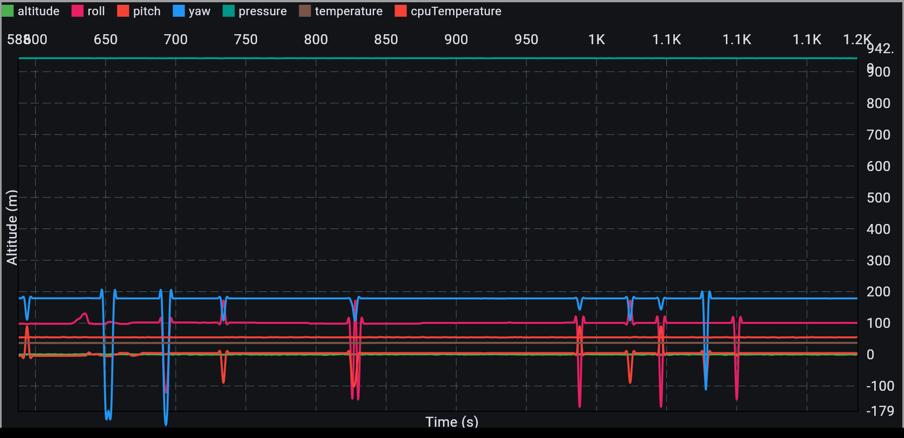
\includegraphics[width=0.8\textwidth]{Imagenes/Bitmap/metrics}
        \caption{Ejemplo del Componente Metrics}
        \label{fig:metrics}
    \end{figure}
    \item \textbf{Attitude:} renderiza un modelo tridimensional que rota en tiempo real según los valores de yaw, pitch y roll incluidos en cada evento, de esta manera es posible ver la orientación actual del CanSat.
    \begin{figure}[H]
        \centering
        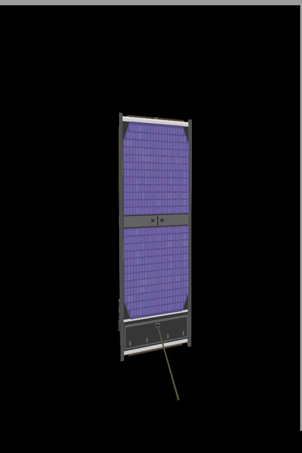
\includegraphics[width=0.4\textwidth]{Imagenes/Bitmap/attitude}
        \caption{Ejemplo del Componente Attitude}
        \label{fig:attitude}
    \end{figure}
    \item \textbf{TelemetryChart:} representa todos los valores de los parámetros recibidos como gráficas temporales utilizando, permitiendo observar la evolución de múltiples variables simultáneamente.
    \begin{figure}[H]
        \centering
        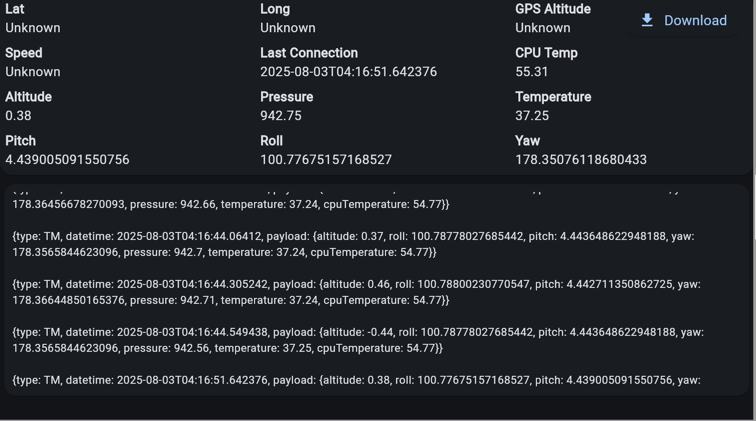
\includegraphics[width=0.8\textwidth]{Imagenes/Bitmap/telemetry_chart}
        \caption{Ejemplo del Componente TelemetryChart}
        \label{fig:telemetry_chart}
    \end{figure}
    \item \textbf{Map:} muestra un mapa con la última ubicación recibida del CanSat.
    \begin{figure}[H]
        \centering
        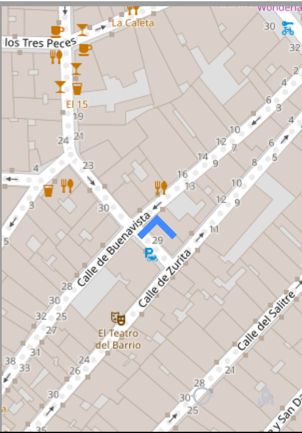
\includegraphics[width=0.4\textwidth]{Imagenes/Bitmap/map}
        \caption{Ejemplo del Componente Map}
        \label{fig:map}
    \end{figure}
    \item \textbf{Camera:} muestra la retransmisión de vídeo en directo.
\end{itemize}
\begin{figure}[H]
    \centering
    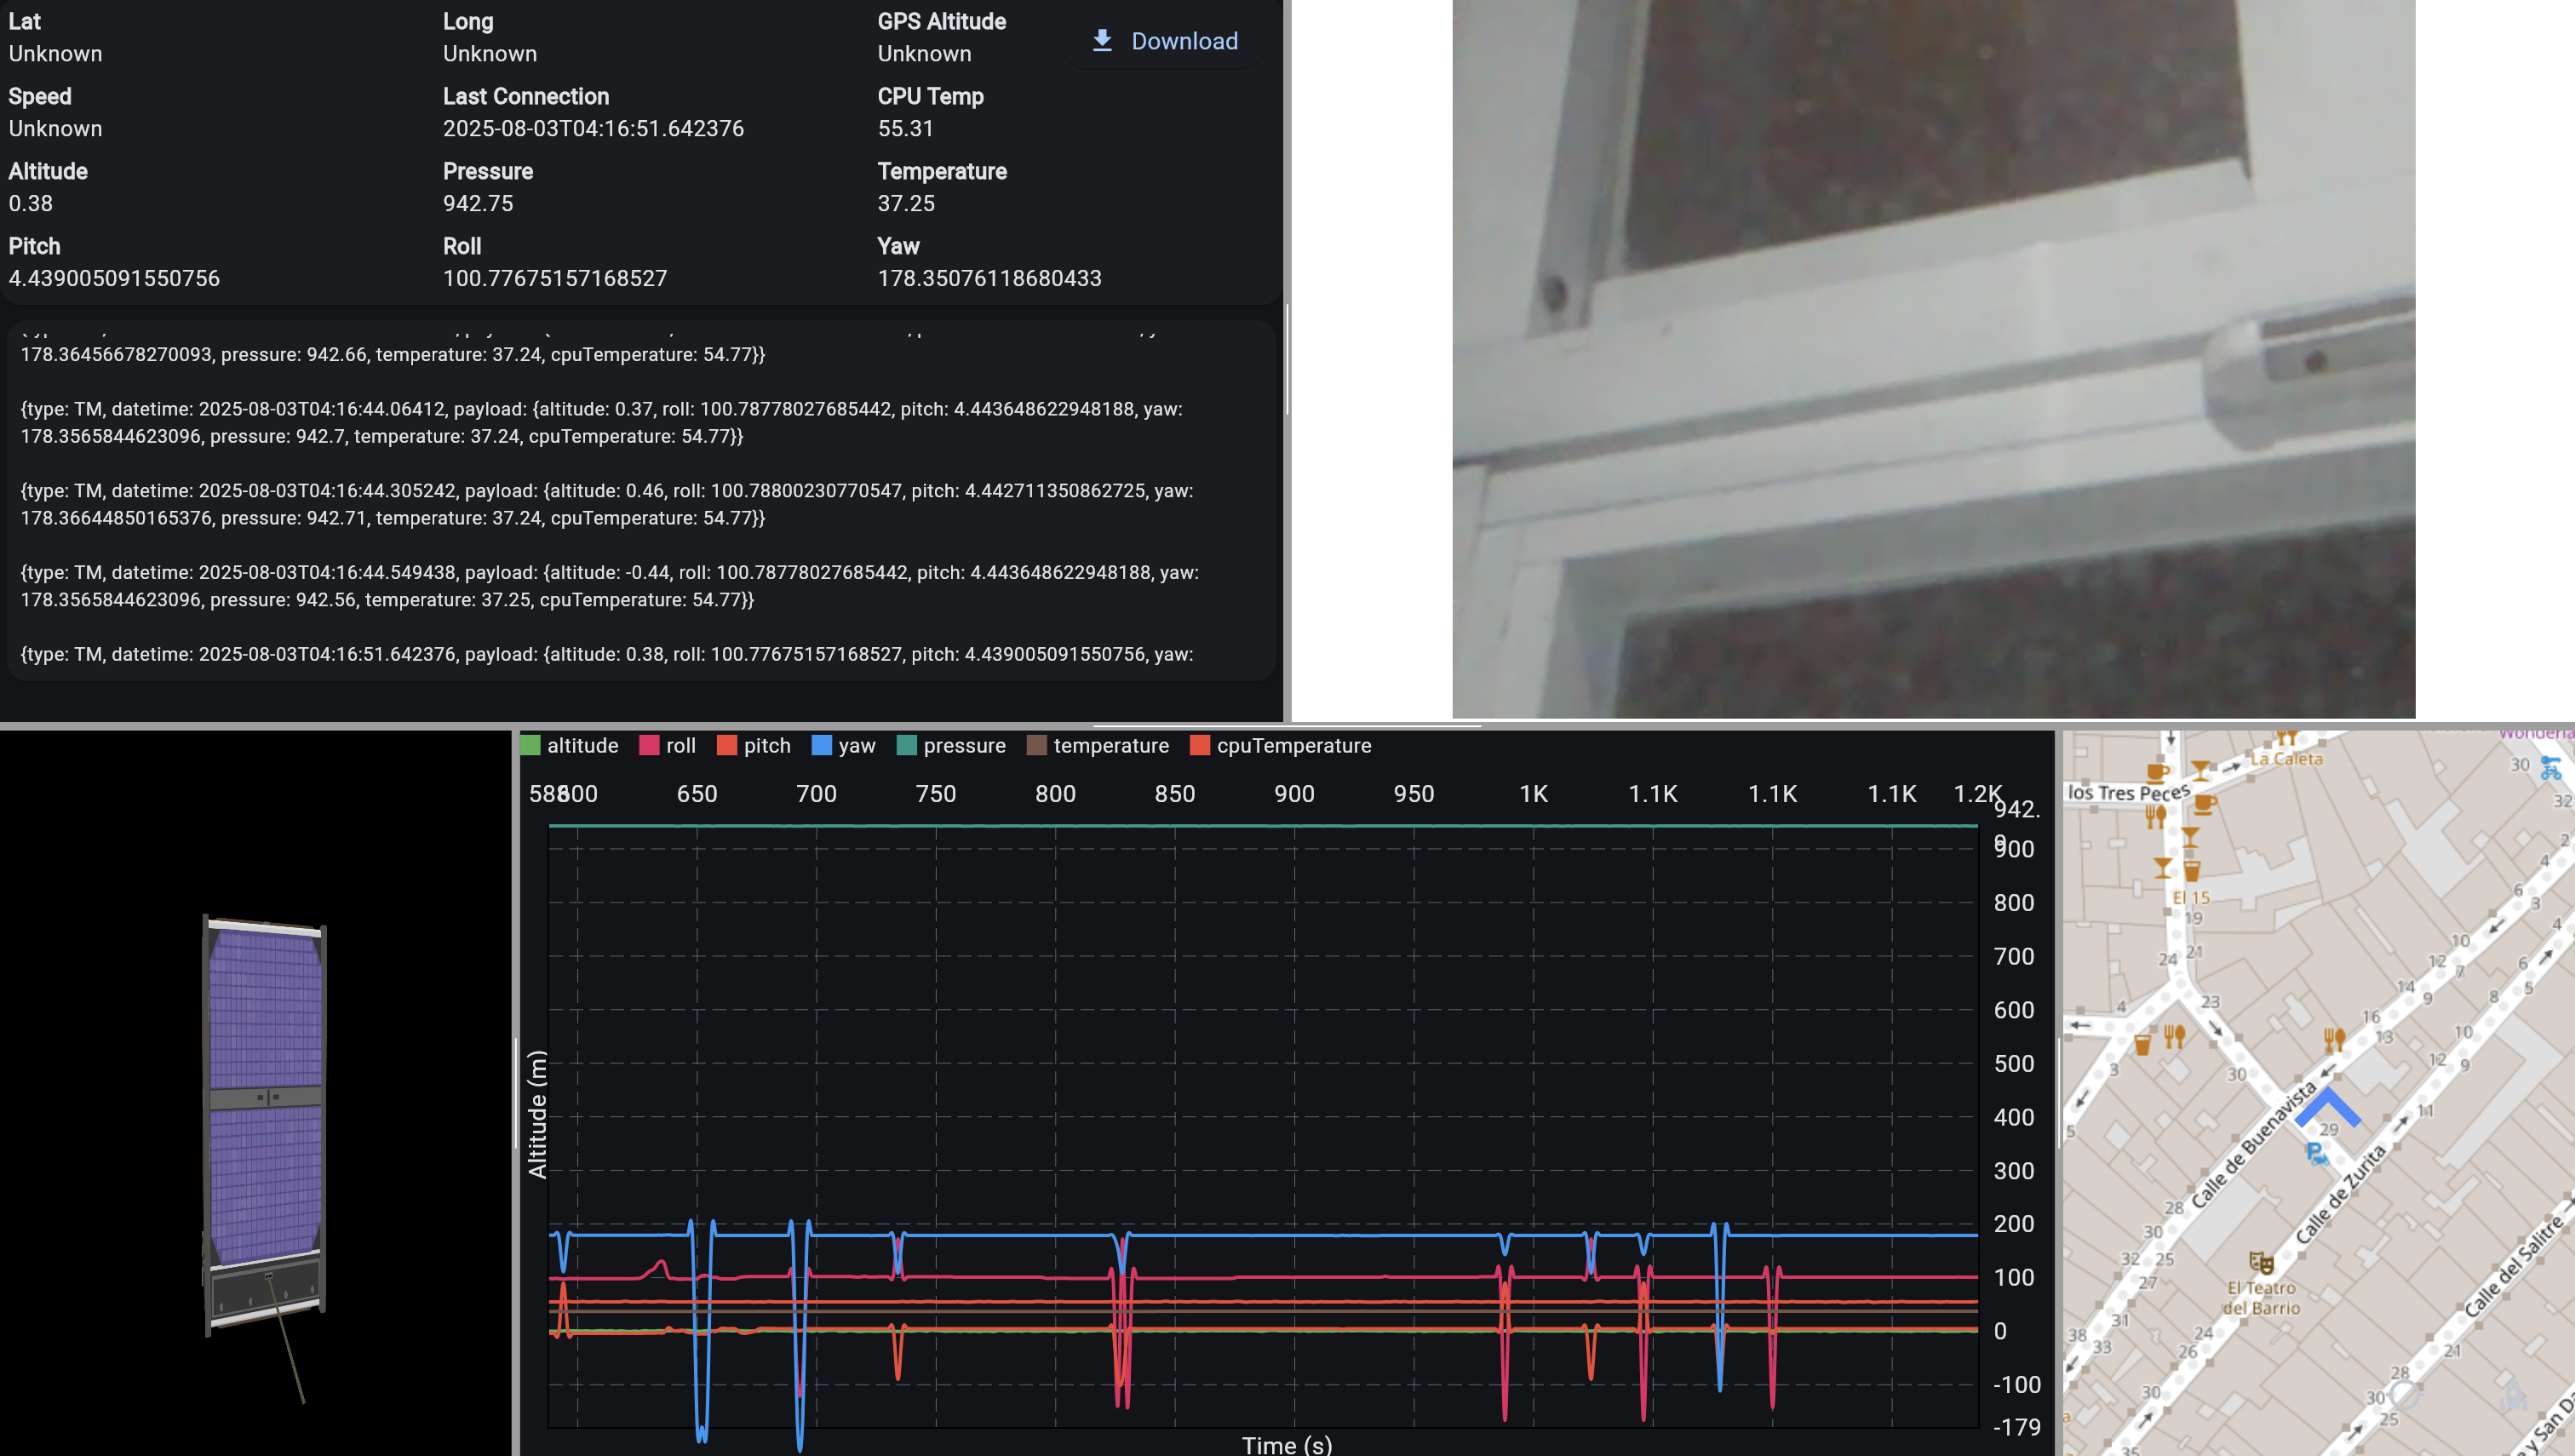
\includegraphics[width=1\textwidth]{Imagenes/Bitmap/initerfaz_general}
    \caption{Interfaz en modo escritorio}
    \label{fig:interfaz_general}
\end{figure}

\subsection{Adaptabilidad}

El diseño de la interfaz se adapta automáticamente a la resolución de pantalla.
En escritorio el espacio se divide en secciones horizontales y verticales que pueden ser redimensionadas de manera independiente, mientras que en móviles los elementos se muestran uno debajo de otro.


\section{Pruebas de integración y validación}

